\chapter[Elicitação]{Elicitação}
A elicitação é uma das atividades fundamentais da Engenharia de Requisitos e consiste no processo de identificar
itens de informação que determinam as características de um sistema. \cite{jitnah} 

Para \citeonline{paetsch} a elicitação de requisitos tem o intuito de descobrir
os requisitos e identificar as fronteiras do sistema, estas definem o contexto, consultando os \textit{stakeholders} (cliente, usuários e desenvolvedores).

A atividade de elicitação pode ser realizada através da aplicação de várias técnicas, como: Grupos focais, entrevistas, questionários,
introspecção, análise de protocolo, prototipagem, animação, análise de cenário, estudo etnográfico, observação, análise de tarefas,
\textit{workshops} e \textit{brainstorming}. (\cite{jitnah} ; \cite{coulin})

\section{Técnicas de Elicitação de Requisitos}
\label{tecnicas}

As técnicas de elicitação de requisitos foram selecionadas de acordo com a interação entre a equipe e o cliente e de acordo com os níveis de conhecimento e de abstração dos requisitos a serem obtidos.
As técnicas escolhidas foram:\\
\begin{itemize}
\item Análise documental;
\item \textit{Workshop} de Requisitos;
\item Entrevistas.
\end{itemize}

\subsection{\textit{Workshop}}
  Foram realizados dois \textit{Workshops} com o intuito de Estabelecer o Tema de Investimento e Levantar Épicos. Nos \textit{Workshops}
  foram definidos papéis para organizar de forma efetiva a reunião. Os papéis e as responsabilidades podem ser vistas abaixo.
  
\textbf{Facilitador:}

	Dirige o \textit{Workshop}
	
	Deixa bem claro o objetivo de cada passo do \textit{Workshop}
	
	Não permite críticas ou debates durante o \textit{Workshop}
		
\textbf{Moderador:}

	Controle do tempo
	
	Manter foco do \textit{Workshop}
	
\textbf{Registrador:}

	Registra o que teve de importante no \textit{Workshop}
	
O primeiro \textit{Workshop} ocorreu com base no planejamento da Figura \ref{fig:workshop1} e foi realizado para entender o problema
da empresa. O segundo \textit{Workshop} foi realizado com o intuito de levantar os épicos e aconteceu conforme o planejamento da Figura
\ref{fig:workshop2}.

\begin{figure}[!htb]
\centering
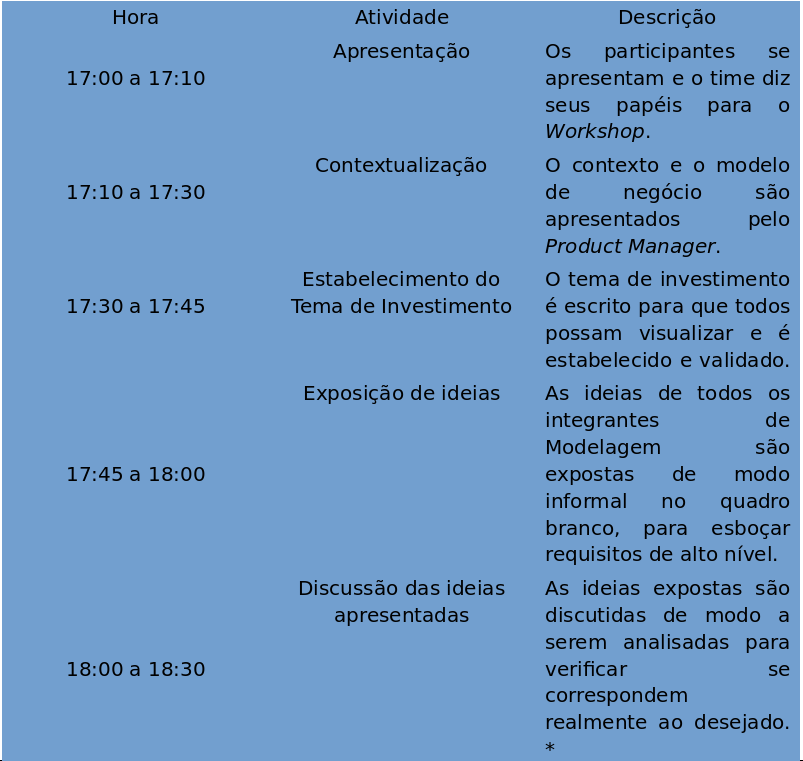
\includegraphics[scale=0.55]{figuras/workshop1.png}
\caption{Planejamento do \textit{Workshop} 1}
\label{fig:workshop1}
\end{figure}

\begin{figure}[!htb]
\centering
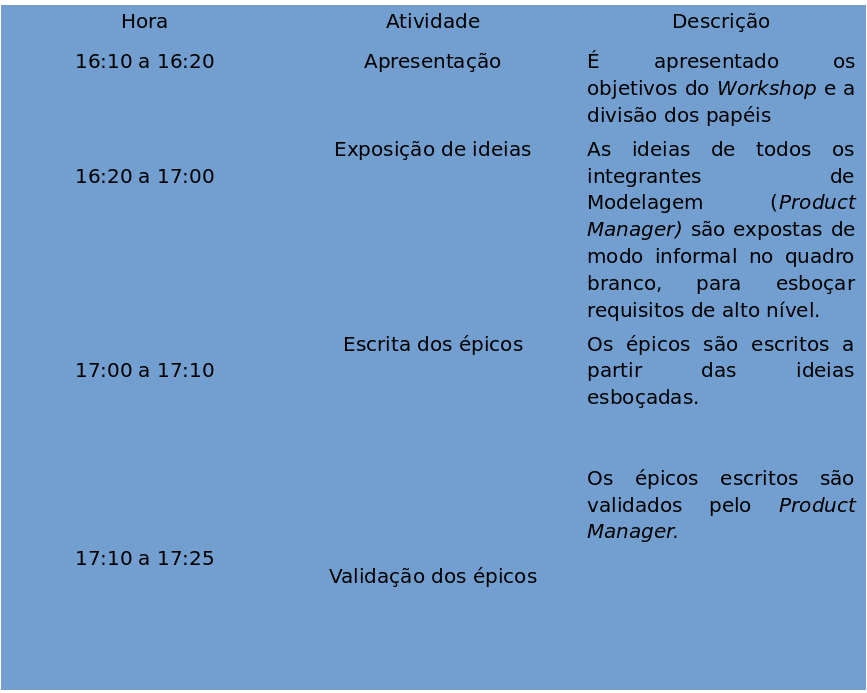
\includegraphics[scale=0.55]{figuras/workshop2.png}
\caption{Planejamento do \textit{Workshop} 2}
\label{fig:workshop2}
\end{figure}

% TRABALHO 1
% A técnica de análise documental será empregada inicialmente, pois permite a visualização de formulários, fichas, relatórios e outros documentos da empresa, podendo auxiliar no entendimento do contexto. ~\cite{falbo}.\\
% 
% Serão realizados um ou mais \textit{Workshops} para levantamento de requisitos em mais alto nível, de acordo com a necessidade de entendimento da equipe e disponibilidade do cliente.
% Segundo \citeonline{nuseibeh}, essa técnica explora a dinâmica em grupo, dessa forma, possibilitando conhecer uma visão geral sobre o problema.\\
% 
% Nos \textit{Workshops} serão atribuídas responsabilidades as pessoas, como a de controlar o tempo da reunião, de fazer anotações e de verificar se a reunião está perdendo o foco, assim como sugerido por ~\cite{falbo}. \\
% 
% Para condução da elicitação nesta técnica, serão considerados os procedimentos relatados por Alexander e Beus-Dukic (2009 apud  \citeonline{falbo}). Dessa forma, as ideias e as necessidades relatadas serão esboçadas em quadro branco para que todos os participantes possam visualizar e opinar sobre as prioridades, os objetivos e diferentes soluções. E por fim um relatório deve ser gerado com todas as informações levantadas no \textit{Workshop}.\\
% 
% Serão realizadas entrevistas para elicitação de requisitos, visto que esse tipo de técnica permite uma compreensão das necessidades e dos requisitos em visões mais específicas, e em um menor nível de abstração que nos \textit{Workshops}. 
% De acordo com \citeonline{coulin}, a entrevista é uma forma rápida de coletar uma grande quantidade de dados. No contexto deste trabalho é uma boa técnica dada a interação que foi estabelecida com o cliente.\\
% 
% As entrevistas podem ser fechadas, abertas ou mistas. As entrevistas fechadas possuem perguntas predefinidas. Já nas entrevistas abertas as perguntas são criadas de acordo com os tópicos explorados. As entrevistas mistas combinam os dois tipos, ou seja, algumas perguntas são definidas anteriormente e de acordo com os assuntos levantados nas reuniões novas perguntas são criadas.~\cite{sommerville}.\\
% 
% Serão realizadas entrevistas mistas, pois como esta técnica será combinada com outras duas, algumas perguntas podem ser predefinidas baseadas nas elicitações realizadas anteriormente e há a possibilidade de criação de novas perguntas.\\
% 
% As entrevistas serão registradas por meio de anotações, embora seja um processo mais lento, favorece uma análise momentânea dos requisitos levantados e assim auxilia na exploração dos tópicos a serem abordados na entrevista.\\
% 
